% Final manuscript, Research Methods and Tools (SE-2414), Astana IT University.
% Build: latexmk -pdf main.tex   (Overleaf: upload the paper/ folder, main document = main.tex)
% All numbers come from generated/numbers.tex, written by `python3 -m paper.analysis.run`.
\documentclass[journal]{IEEEtran}


\usepackage[utf8]{inputenc}
\usepackage[english]{babel}
\usepackage{amsmath}
\usepackage{graphicx}
\usepackage{booktabs}
\usepackage{array}
\usepackage{multirow}
\usepackage{xcolor}
\usepackage{tikz}
\usetikzlibrary{arrows.meta,positioning,fit,backgrounds,calc}
\usepackage[hidelinks]{hyperref}
\usepackage{cite}
\usepackage{url}

% Cyrillic examples: \kk{Cyrillic}{transliteration}. Overleaf has T2A fonts and prints the Cyrillic;
% a TeX installation without them falls back to the transliteration.
\newif\ifcyrillic
\IfFileExists{t2aenc.def}{\cyrillictrue}{\cyrillicfalse}
\ifcyrillic
  \usepackage[T2A,T1]{fontenc}
  \newcommand{\kk}[2]{{\fontencoding{T2A}\selectfont #1}}
\else
  \usepackage[T1]{fontenc}
  \newcommand{\kk}[2]{\textit{#2}}
\fi

\definecolor{kkblue}{HTML}{0072B2}
\definecolor{enorange}{HTML}{E69F00}
\definecolor{pend}{HTML}{8C8C8C}

% Generated by paper/analysis/run.py from the saved logs. Do not edit by hand.
\newcommand{\AblBleuGapFull}{-17.84}
\newcommand{\AblBleuGapK}{-13.24}
\newcommand{\AblBleuRedPct}{26}
\newcommand{\AblChrfGapK}{-9.00}
\newcommand{\AblFoneGapFull}{-22.01}
\newcommand{\AblFoneGapK}{-14.28}
\newcommand{\AblFoneRedPct}{35}
\newcommand{\CharRatio}{1.05}
\newcommand{\CovGemini}{276}
\newcommand{\CovGemma}{0}
\newcommand{\CovNLLB}{0}
\newcommand{\CovPct}{33.3}
\newcommand{\CovQwen}{0}
\newcommand{\DictBleuEN}{0.83}
\newcommand{\DictBleuKK}{0.93}
\newcommand{\DictChrfEN}{1.70}
\newcommand{\DictChrfGap}{0.78}
\newcommand{\DictChrfGapHi}{1.15}
\newcommand{\DictChrfGapLo}{0.44}
\newcommand{\DictChrfKK}{2.48}
\newcommand{\GapNoLatin}{-7.28}
\newcommand{\GapNoLatinHi}{-4.27}
\newcommand{\GapNoLatinLo}{-10.00}
\newcommand{\GapNoPilot}{-8.91}
\newcommand{\GapNoPilotHi}{-5.48}
\newcommand{\GapNoPilotLo}{-12.51}
\newcommand{\GemBleuEN}{38.70}
\newcommand{\GemBleuENHi}{42.00}
\newcommand{\GemBleuENLo}{35.38}
\newcommand{\GemBleuGap}{-17.84}
\newcommand{\GemBleuGapAbs}{17.84}
\newcommand{\GemBleuGapHi}{-13.84}
\newcommand{\GemBleuGapLo}{-21.83}
\newcommand{\GemBleuKK}{20.86}
\newcommand{\GemBleuKKHi}{23.42}
\newcommand{\GemBleuKKLo}{18.40}
\newcommand{\GemChrfEN}{65.33}
\newcommand{\GemChrfENHi}{67.58}
\newcommand{\GemChrfENLo}{63.13}
\newcommand{\GemChrfGap}{-8.93}
\newcommand{\GemChrfGapAbs}{8.93}
\newcommand{\GemChrfGapHi}{-5.64}
\newcommand{\GemChrfGapLo}{-12.19}
\newcommand{\GemChrfKK}{56.40}
\newcommand{\GemChrfKKHi}{58.68}
\newcommand{\GemChrfKKLo}{54.11}
\newcommand{\GemChrfPPEN}{63.37}
\newcommand{\GemChrfPPENHi}{65.74}
\newcommand{\GemChrfPPENLo}{61.07}
\newcommand{\GemChrfPPGap}{-11.28}
\newcommand{\GemChrfPPGapAbs}{11.28}
\newcommand{\GemChrfPPGapHi}{-7.92}
\newcommand{\GemChrfPPGapLo}{-14.50}
\newcommand{\GemChrfPPKK}{52.09}
\newcommand{\GemChrfPPKKHi}{54.40}
\newcommand{\GemChrfPPKKLo}{49.88}
\newcommand{\GemRelGapPct}{13.7}
\newcommand{\GemTerEN}{48.29}
\newcommand{\GemTerENHi}{51.77}
\newcommand{\GemTerENLo}{44.64}
\newcommand{\GemTerGap}{18.55}
\newcommand{\GemTerGapAbs}{18.55}
\newcommand{\GemTerGapHi}{23.02}
\newcommand{\GemTerGapLo}{13.93}
\newcommand{\GemTerKK}{66.84}
\newcommand{\GemTerKKHi}{70.13}
\newcommand{\GemTerKKLo}{63.34}
\newcommand{\ItemsBelow}{91}
\newcommand{\ItemsBelowPct}{65.9}
\newcommand{\KPrimary}{5}
\newcommand{\LabLexical}{9}
\newcommand{\LabMorphological}{1}
\newcommand{\LabReferenceMismatch}{13}
\newcommand{\LabScript}{3}
\newcommand{\LabSemantic}{4}
\newcommand{\LatEN}{0.91}
\newcommand{\LatKK}{1.04}
\newcommand{\LenCutHi}{23}
\newcommand{\LenCutLo}{19}
\newcommand{\NAnyLatin}{24}
\newcommand{\NBoot}{1,000}
\newcommand{\NItems}{430}
\newcommand{\NMostlyLatin}{3}
\newcommand{\NNoLatin}{135}
\newcommand{\NNoPilot}{124}
\newcommand{\NPairs}{138}
\newcommand{\NPilotOverlap}{14}
\newcommand{\NPromptsPerModel}{830}
\newcommand{\NQa}{200}
\newcommand{\NRefLatin}{16}
\newcommand{\NResponses}{276}
\newcommand{\NReviewed}{30}
\newcommand{\NmCtrlEN}{0.1}
\newcommand{\NmCtrlKK}{0.4}
\newcommand{\NmDiff}{7.9}
\newcommand{\NmDiffHi}{9.1}
\newcommand{\NmDiffLo}{6.7}
\newcommand{\NmEN}{2.5}
\newcommand{\NmENHi}{3.1}
\newcommand{\NmENLo}{2.0}
\newcommand{\NmKK}{10.5}
\newcommand{\NmKKHi}{11.7}
\newcommand{\NmKKLo}{9.2}
\newcommand{\NmShareOfMissEN}{8.6}
\newcommand{\NmShareOfMissKK}{20.6}
\newcommand{\QaAEN}{19.5}
\newcommand{\QaAENonly}{0}
\newcommand{\QaAKK}{19.5}
\newcommand{\QaAKKonly}{0}
\newcommand{\QaAP}{1.0000}
\newcommand{\QaRndEN}{27.0}
\newcommand{\QaRndENonly}{46}
\newcommand{\QaRndKK}{18.5}
\newcommand{\QaRndKKonly}{29}
\newcommand{\QaRndP}{0.0639}
\newcommand{\RecallEN}{70.7}
\newcommand{\RecallKK}{49.2}
\newcommand{\RhoLenEN}{-0.09}
\newcommand{\RhoLenKK}{-0.15}
\newcommand{\RhoTok}{0.11}
\newcommand{\RhoTokP}{0.21}
\newcommand{\TokCharPrem}{2.02}
\newcommand{\TokCharPremHi}{2.08}
\newcommand{\TokCharPremLo}{1.97}
\newcommand{\TokPerCharEN}{20.3}
\newcommand{\TokPerCharKK}{41.1}
\newcommand{\TokRatio}{2.12}
\newcommand{\TokRatioHi}{2.19}
\newcommand{\TokRatioLo}{2.05}
\newcommand{\TokSrcRatio}{2.11}
\newcommand{\WilMed}{-6.90}
\newcommand{\WilP}{2.1\times10^{-6}}
\newcommand{\WilR}{-0.47}
\newcommand{\WilW}{2564}


\newcommand{\gap}{\ensuremath{\Delta}}
\newcommand{\ENKK}{EN$\rightarrow$KK}
\newcommand{\KKEN}{KK$\rightarrow$EN}

\hyphenation{Ka-zakh chrF Be-le-be-le Kaz-ParC}

\begin{document}

\title{Kazakh--English Performance Gaps in Large Language Models: A Paired Benchmark with Morphology- and Tokenization-Aware Diagnostics}

\author{Birkhanym~Kazhymukhamet,
        Meruert~Khaigeldinova,
        and~Dana~Bekbosyn%
\thanks{The authors are with the School of Software Engineering, Astana IT University, Astana 010000, Kazakhstan.}%
\thanks{Corresponding author: B.~Kazhymukhamet (e-mail: [corresponding e-mail]).}}

\markboth{Kazhymukhamet \MakeLowercase{\textit{et al.}}: Kazakh--English Performance Gaps in Large Language Models}%
{Kazhymukhamet \MakeLowercase{\textit{et al.}}: Kazakh--English Performance Gaps in Large Language Models}

\maketitle

\begin{abstract}
\textit{Background:} Large language models (LLMs) are widely used for Kazakh, an agglutinative Turkic language with limited training data, yet their reliability is rarely measured on content held constant across Kazakh and English.
\textit{Aim:} We quantify how LLM translation quality differs between the two target languages and identify measurable sources of the difference.
\textit{Method:} We release KAZLLM, a hash-frozen benchmark of \NItems{} paired items (\NPromptsPerModel{} prompts per model) drawn from FLORES-200, KazParC, Belebele and team-written probes, together with an open pipeline that rejects simulated outputs. This report analyses \NResponses{} saved responses of Gemini 3.5 Flash-Lite covering \NPairs{} FLORES-200 sentences translated in both directions. Uncertainty is estimated with \NBoot{} paired bootstrap resamples and Holm-corrected signed-rank tests.
\textit{Results:} Translation into Kazakh scored \GemChrfKK{} chrF2 against \GemChrfEN{} into English, a gap of $\GemChrfGap$ points (95\% CI $[\GemChrfGapLo, \GemChrfGapHi]$); \ItemsBelowPct\% of items scored lower into Kazakh. The gap persisted under chrF++, BLEU and TER and after removing pilot items or Latin-script outputs. Same-stem, different-ending matches accounted for \NmKK\% of Kazakh reference words versus \NmEN\% of English ones, and Kazakh outputs used \TokRatio$\times$ as many tokens for \CharRatio$\times$ as many characters.
\textit{Conclusion:} Lower quality into Kazakh is robust for this model, and suffix-level mismatch and tokenization cost are measurable contributors; question answering, further models and blind human annotation remain to be completed with the released pipeline.
\end{abstract}

\begin{IEEEkeywords}
Machine translation, low-resource languages, agglutinative morphology, chrF, paired bootstrap, Turkic languages.
\end{IEEEkeywords}

\section{Introduction}
\label{sec:intro}

\IEEEPARstart{L}{arge} language models (LLMs) are now the default writing and translation assistants for many people who work in more than one language. In Kazakhstan, students, translators, journalists and public bodies routinely ask general-purpose LLMs to translate between Kazakh and English or to answer questions about Kazakh text. Kazakh is the state language of the country, but in the vocabulary of language technology it is a low- to mid-resource language: it has comparatively little curated digital text, a Cyrillic script that is shared with Russian, and an agglutinative morphology in which a single word can carry a stem followed by plural, possessive, case and other suffixes chosen by vowel harmony~\cite{joshi2020state,mirzakhalov2021turkic}. Each of these properties is a plausible reason why a model trained mostly on English could perform worse when it must \emph{produce} Kazakh.

Evidence that such a disadvantage exists comes from three directions. First, multilingual benchmarking of generative models reports systematically lower scores for lower-resource languages~\cite{ahuja2023mega,lai2023beyond}, and large translation studies find that general LLMs approach dedicated systems for high-resource languages but lag for low-resource ones~\cite{robinson2023chatgpt,zhu2024multilingual}. Second, Kazakh-specific evaluations reach the same conclusion: KazMMLU shows that even strong models struggle on Kazakh knowledge questions and that accuracy depends heavily on the prompt language~\cite{togmanov2025kazmmlu}, a pilot evaluation of seven LLMs documents weaknesses on Kazakh tasks~\cite{maxutov2024kazakh}, and the KazParC corpus study reports weaker scores for translation into Kazakh than into Russian~\cite{yeshpanov2024kazparc}. Third, the inequality begins before any text is generated: commercial tokenizers need several times more tokens to encode the same content in many non-English languages, which raises cost and shortens the usable context~\cite{petrov2023tokenizer,ahia2023cost}.

These studies, however, leave a specific gap. Each isolates one symptom---subject knowledge, corpus-level translation quality, or token counts---and none measures the \emph{same} items in Kazakh and English for a general-purpose LLM while also asking \emph{which measurable properties of the output} accompany the difference. KazMMLU has no English counterpart, the KazParC evaluation compares dedicated translation systems rather than LLMs, and tokenizer studies measure input length rather than output quality. The explanation most often offered, that agglutinative morphology is to blame, has been suggested but rarely tested~\cite{yeshpanov2024kazparc}. Without paired measurements, a lower Kazakh score cannot be separated from differences in item difficulty, and without diagnostics it cannot inform users or developers about what goes wrong.

This article addresses that gap with a paired, within-item design. Our research question, fixed in the study protocol, is: \emph{How does the accuracy of selected LLMs on Kazakh-language translation and question-answering tasks compare with their accuracy on equivalent English-language tasks, and which types of linguistic error are associated with any differences observed?} We hypothesised that performance is lower in Kazakh (H1) and that morphological errors make up the largest share of Kazakh errors (H2).

The study was designed for three LLMs, a dedicated translation baseline and blind human annotation. At the time of writing, the saved evidence covers one model, Gemini 3.5 Flash-Lite, on \NPairs{} FLORES-200 sentences translated in both directions (\NResponses{} of \NPromptsPerModel{} planned responses for that model). We therefore answer the translation part of the question for this model with full statistical rigour, test morphology-related explanations with automatic, controlled diagnostics rather than with human labels, and report the remaining conditions transparently as pending. All of them can be completed with the released pipeline without changing the protocol.

The contributions of this article are as follows.
\begin{enumerate}
\item \textbf{A paired Kazakh--English benchmark and an auditable pipeline.} KAZLLM contains \NItems{} items (\NPromptsPerModel{} prompts per model) from FLORES-200, KazParC and Belebele, plus 30 team-written probes covering six Kazakh phenomena. Inputs are frozen by SHA-256 hashes, every saved response carries its prompt hash and raw API record, and the scorer refuses incomplete or simulated runs.
\item \textbf{A rigorous directional comparison.} On \NPairs{} paired items, translation into Kazakh is $\GemChrfGapAbs$ chrF2 points worse than translation into English, with a paired bootstrap interval that excludes zero and a consistent direction across four metrics and three sensitivity analyses.
\item \textbf{Controlled diagnostics of the gap.} We introduce an inflection-tolerant prefix analysis with a mismatched-reference control and a truncation ablation, an automatic script audit, and an analysis of API-reported token usage. Together they show that suffix-level mismatch and tokenization cost are measurable contributors, whereas script errors explain only a small part of the gap.
\item \textbf{Transparent reporting.} Every number in the article is generated from the saved logs by one command, and all protocol deviations and pending conditions are documented.
\end{enumerate}

The rest of the article is organised as follows. Section~\ref{sec:related} synthesises related work, Section~\ref{sec:methods} describes the design, data and analysis, Section~\ref{sec:results} reports the results, Section~\ref{sec:discussion} interprets them and discusses threats to validity, and Section~\ref{sec:conclusion} concludes.

\section{Related Work}
\label{sec:related}

We organise prior work into four themes: how general LLMs perform on lower-resource languages, what is known about Kazakh specifically, how tokenization and morphology interact with model quality, and how translation evaluation should be designed and reported. Table~\ref{tab:closest} compares the studies closest to ours.

\subsection{LLMs and Lower-Resource Languages}
Evaluations of generative models across many languages consistently find that performance tracks the amount of available data. MEGA evaluated several generative models on multilingual benchmarks and reported large drops for lower-resource languages and non-Latin scripts~\cite{ahuja2023mega}. Lai et al.\ extended this to dozens of tasks and languages and reached a similar conclusion~\cite{lai2023beyond}. For translation in particular, Robinson et al.\ translated FLORES-200 into more than 200 languages with GPT models and found that a language's resource level was the strongest predictor of how far the LLM fell behind dedicated systems~\cite{robinson2023chatgpt}. Zhu et al.\ evaluated eight LLMs in both translation directions on FLORES-101 and showed that even GPT-4 trails strong commercial systems for low-resource directions~\cite{zhu2024multilingual}, and Hendy et al.\ observed that GPT models are competitive for high-resource pairs while weaker elsewhere~\cite{hendy2023good}. These studies establish that a gap is expected but are broad by design: Kazakh appears, if at all, as one of many languages, and the analyses stop at corpus scores.

\subsection{Kazakh Resources and Evaluations}
Kazakh has gained dedicated resources in recent years. FLORES-101 and its successor FLORES-200 provide professionally translated, multi-way parallel evaluation sentences~\cite{goyal2022flores,nllb2022}; Belebele adds parallel multiple-choice reading comprehension questions built on the same passages~\cite{bandarkar2024belebele}; and KazParC contributes a large Kazakh-centred parallel corpus with an evaluation of translation systems~\cite{yeshpanov2024kazparc}. Earlier work on Turkic languages documented the scarcity of parallel data and the difficulty of translating into agglutinative targets~\cite{mirzakhalov2021turkic}, and Kazakh--English neural translation has been improved with back-translation and transfer learning~\cite{karyukin2023nmt} and with part-of-speech features~\cite{yazar2025kazakh}. Task-specific Kazakh systems, such as geographical question answering, have also been built~\cite{mukanova2024geoqa}. For LLMs, KazMMLU measures knowledge in Kazakh and Russian and shows a strong effect of prompt language~\cite{togmanov2025kazmmlu}, while Maxutov et al.\ piloted seven LLMs on Kazakh tasks~\cite{maxutov2024kazakh}. Parameter-efficient fine-tuning has been proposed to improve LLM translation for low-resource languages~\cite{liang2025lsftl}. None of these studies holds content constant across Kazakh and English for the same LLM, and none links the size of a Kazakh deficit to measurable properties of the generated text.

\subsection{Tokenization and Morphology}
Tokenizers trained on English-dominated corpora split many other languages into more pieces. Petrov et al.\ measured the resulting length disparities across many tokenizers, with Kazakh among the languages needing several times more tokens than English for parallel text~\cite{petrov2023tokenizer}, and Ahia et al.\ showed that such disparities translate into higher prices and worse utility for users of commercial APIs~\cite{ahia2023cost}. Rust et al.\ found that the quality of a multilingual tokenizer for a given language is associated with downstream performance in that language~\cite{rust2021tokenizer}. For agglutinative languages, morphology is a natural suspect: a missed or wrong suffix changes one word form while leaving the stem intact. The KazParC authors suggested this explanation for weaker scores into Kazakh but did not test it~\cite{yeshpanov2024kazparc}. Our diagnostics are designed to provide such a test with automatic, reproducible measurements.

\subsection{Evaluation Methodology}
Character-level metrics are preferred for morphologically rich targets because they give partial credit for related word forms: chrF~\cite{popovic2015chrf} and its word-augmented variant chrF++~\cite{popovic2017chrfpp} correlate better with human judgements than BLEU~\cite{papineni2002bleu} in large meta-evaluations~\cite{kocmi2021ship}. TER provides an edit-based view~\cite{snover2006ter}, and sacreBLEU standardises tokenization and signatures so that scores are comparable~\cite{post2018sacrebleu}. Statistical practice in translation research is often weak: Marie et al.\ found that most papers reported no significance testing~\cite{marie2021credibility}, while paired bootstrap resampling~\cite{koehn2004significance} and careful test selection~\cite{dror2018hitchhiker} remain the recommended remedies. Expert error annotation in the MQM framework~\cite{lommel2014mqm,freitag2021experts} is the reference standard for explaining score differences, and benchmark contamination is an increasing concern for public test sets~\cite{sainz2023contamination}. Our design follows these recommendations and states explicitly where it falls short.

\begin{table*}[!t]
\centering
\caption{Comparison of the Most Closely Related Studies. ``Paired'' Means That the Same Items Are Scored in Both Language Conditions.}
\label{tab:closest}
\footnotesize
\begin{tabular}{@{}p{3.1cm}p{2.6cm}p{3.0cm}p{1.6cm}p{5.6cm}@{}}
\toprule
Study & Languages & Systems & Paired KK/EN & Analysis beyond corpus scores \\
\midrule
Robinson et al.\ 2023~\cite{robinson2023chatgpt} & 200+ incl.\ Kazakh & ChatGPT, GPT-4, NLLB, Google & No & Resource-level predictors of the LLM deficit \\
Zhu et al.\ 2024~\cite{zhu2024multilingual} & 102 incl.\ Kazakh & 8 LLMs, NLLB, M2M & Directions only & In-context learning behaviour \\
Petrov et al.\ 2023~\cite{petrov2023tokenizer} & Many incl.\ Kazakh & Tokenizers only & n/a & Token-length disparity; no output quality \\
Yeshpanov et al.\ 2024~\cite{yeshpanov2024kazparc} & KK, EN, RU, TR & Dedicated MT systems & No & Morphology suggested, not tested \\
Maxutov et al.\ 2024~\cite{maxutov2024kazakh} & Kazakh & 7 LLMs & No & Task-level comparison of models \\
Togmanov et al.\ 2025~\cite{togmanov2025kazmmlu} & KK, RU & Open and proprietary LLMs & No (KK vs.\ RU) & Prompt language, confidence, negation \\
\textbf{This work} & KK, EN & Gemini 3.5 Flash-Lite (+3 pending) & \textbf{Yes} & Prefix near-miss with control, truncation ablation, script audit, API token usage \\
\bottomrule
\end{tabular}
\end{table*}

\section{Materials and Methods}
\label{sec:methods}

\subsection{Study Design}
The study is a quantitative, paired within-item benchmark (Fig.~\ref{fig:design}). Every item exists in a Kazakh and an English version with the same content, and every model receives both versions under identical English instructions. The language condition is therefore the only factor that changes within a pair, so differences between conditions cannot be attributed to item difficulty. For translation, the language condition is the translation direction: English to Kazakh (\ENKK) or Kazakh to English (\KKEN). For question answering (QA), it is the language of the passage, question and options. The unit of analysis is one saved model response to one prompt.

\begin{figure*}[!t]
\centering
\begin{tikzpicture}[
  font=\footnotesize,
  box/.style={draw, rounded corners=2pt, align=center, minimum height=1.05cm, fill=#1},
  w/.style={text width=#1}, w/.default={2.35cm},
  box/.default={kkblue!8},
  arr/.style={-{Latex[length=2mm]}, thick, draw=black!70},
  lab/.style={font=\scriptsize\itshape, text=black!60}]
\node[box=black!5, w] (data) {\textbf{Frozen inputs}\\FLORES-200 140, KazParC 60, Belebele 200, probes 30};
\node[box, w, right=0.55cm of data] (prompts) {\textbf{Prompt builder}\\830 prompts/model, identical EN instructions};
\node[box, w, right=0.55cm of prompts] (run) {\textbf{Model runners}\\$T{=}0$, seed 42, hashed records};
\node[box, w, right=0.55cm of run] (score) {\textbf{Scoring}\\chrF2, chrF++, BLEU, TER; QA accuracy};
\node[box=enorange!12, w, right=0.55cm of score] (stats) {\textbf{Inference}\\paired bootstrap, Wilcoxon + Holm, McNemar};
\node[box=black!5, below=0.7cm of run, xshift=-1.3cm] (sys) {\textbf{Systems}\\Gemini 3.5 Flash-Lite (\CovGemini/830 saved)\\ \textcolor{pend}{Qwen 2.5 1.5B, Gemma 3, NLLB-200: pending}};
\node[box=enorange!12, below=0.7cm of score, xshift=1.6cm] (diag) {\textbf{Diagnostics}\\script audit $\cdot$ prefix near-miss with control\\truncation ablation $\cdot$ API token usage};
\draw[arr] (data) -- (prompts);
\draw[arr] (prompts) -- (run);
\draw[arr] (run) -- (score);
\draw[arr] (score) -- (stats);
\draw[arr] (run.south |- sys.north) -- (run.south);
\draw[arr] (score.south) -- (score.south |- diag.north);
\node[lab, above=0.05cm of data] {SHA-256 manifest};
\node[lab, above=0.05cm of run] {resumable, no simulation};
\node[lab, above=0.05cm of stats] {seed 42, 1{,}000 resamples};
\end{tikzpicture}
\caption{Study pipeline. Grey boxes are inputs and systems, blue boxes are deterministic processing stages, and orange boxes are the statistical analysis and diagnostics. Every stage reads only saved files, and one command regenerates all reported numbers.}
\label{fig:design}
\end{figure*}

\subsection{Benchmark}
Table~\ref{tab:data} summarises the KAZLLM benchmark. Translation items come from the FLORES-200 \emph{devtest} split, whose sentences were written in English and professionally translated into Kazakh~\cite{goyal2022flores,nllb2022}, and from KazParC~\cite{yeshpanov2024kazparc}, which adds sentence pairs from Kazakh-centred sources. FLORES items carry a source domain (Wikinews, Wikibooks or Wikivoyage). QA items are four-option questions from Belebele~\cite{bandarkar2024belebele}, aligned across the Kazakh Cyrillic and English versions by passage link and question number. The 30 probes were written by the authors to test six phenomena with five sentences each: word order, case marking, possessive marking, negation, tense and aspect, and question formation. Items were selected with a fixed seed (42); translation pairs had to contain 5--40 English words, contain letters in both languages, and contain no URLs or duplicates. The benchmark file and the pilot file are frozen by SHA-256 hashes, and the prompt builder verifies a hash of all generated prompts before any run.

\begin{table}[!t]
\centering
\caption{Composition of the KAZLLM Benchmark}
\label{tab:data}
\footnotesize
\begin{tabular}{@{}llrr@{}}
\toprule
Task & Source & Items & Prompts \\
\midrule
Translation & FLORES-200 devtest & 140 & 280 \\
Translation & KazParC & 60 & 120 \\
Question answering & Belebele & 200 & 400 \\
Probes (\ENKK) & Team-written & 30 & 30 \\
\midrule
Total & & 430 & 830 \\
\bottomrule
\end{tabular}
\end{table}

\subsection{Systems and Generation Settings}
The frozen protocol originally named GPT-4o, Llama~3.1~70B and Gemini~1.5~Pro. Because the study had no paid API budget and a laptop with 8~GB of memory, the lineup was revised before data collection to Gemini 3.5 Flash-Lite through the Google Gemini API (returned model version \texttt{3.5-flash-lite-07-2026}) and two locally run open models, Qwen~2.5~1.5B~\cite{qwen2025tech} and Gemma~3~\cite{gemma2025tech}, through Ollama. An earlier Gemini 2.5 Flash-Lite configuration returned HTTP 404 errors during generation and was replaced before any benchmark response was saved; its configuration is archived in the repository.

All requests used zero-shot prompts with fixed English instructions (``Translate the following \{source\} sentence into \{target\}. Output only the translation.''), temperature 0 and seed 42. Gemini used the minimal thinking level and output budgets of 2{,}048 tokens for translation and 512 for QA. Each saved record stores the prompt identifier, the prompt hash, the request hash, the requested and returned model names, timestamps, elapsed time and the raw API response, including the token counts reported by the service. Collection took place on 10~November 2026 (01:56--15:03 Almaty time, including pauses) and stopped after \CovGemini{} responses because of repeated connection resets; the runner resumes from saved records and never fills gaps with simulated text. The responses were collected in benchmark order, so the saved set consists of the first \NPairs{} complete FLORES-200 pairs.

\subsection{Metrics}
The primary metric is corpus-level chrF2 (character n-grams up to order 6, $\beta=2$)~\cite{popovic2015chrf}, chosen in the protocol because character overlap gives partial credit to inflected forms and does not depend on a word tokenizer. Secondary metrics are chrF++ (adding word bigrams)~\cite{popovic2017chrfpp}, BLEU~\cite{papineni2002bleu} and TER~\cite{snover2006ter}, all computed with sacreBLEU~2.6.0 default signatures and one reference~\cite{post2018sacrebleu}. For a metric $m$, the directional gap is
\begin{equation}
\gap_m = m(\text{\ENKK}) - m(\text{\KKEN}),
\label{eq:gap}
\end{equation}
so that negative values indicate lower quality when the model writes Kazakh (for TER, where lower is better, positive values indicate the same). Model outputs were stripped only of wrappers such as code fences or a leading ``Translation:'' label; their content was never edited. QA accuracy is the share of items whose parsed answer letter equals the gold option; unparsable answers count as wrong.

\subsection{Baselines}
A dictionary baseline substitutes 48 high-frequency word forms and copies all other tokens; it uses no learned parameters and is evaluated on exactly the same items. It is a deliberately low bar that checks whether the LLM outputs carry translation signal at all. The strong translation baseline specified in the protocol is NLLB-200 distilled 600M~\cite{nllb2022,nllb2024nature}, a dedicated multilingual translation model; it is needed to separate an LLM-specific gap from a gap that any system would show into Kazakh. Its runner is included but its outputs are pending. For QA, two rules that ignore language provide calibration: always answering~A, and seeded uniform random guessing.

\subsection{Statistical Analysis}
Uncertainty for corpus scores and gaps is estimated with a paired percentile bootstrap~\cite{koehn2004significance}: \NBoot{} resamples of whole items, drawn once with seed 42 and reused for every quantity, so that both directions of an item always enter a resample together. Sentence-level chrF2 differences are tested with two-sided Wilcoxon signed-rank tests~\cite{wilcoxon1945}, reporting the matched-pairs rank-biserial correlation $r_{\mathrm{rb}}$ as effect size and a Holm correction across the three planned comparisons~\cite{holm1979}. Paired QA outcomes are compared with the exact McNemar test~\cite{mcnemar1947} and exact Clopper--Pearson intervals~\cite{clopper1934}. H1 for translation is supported if the 95\% interval of $\gap_{\mathrm{chrF2}}$ lies below zero and, once NLLB outputs exist, below the NLLB gap. Subgroup analyses by domain and source length are exploratory and are not corrected for multiplicity.

\subsection{Diagnostics}
\paragraph*{Script audit} For every Kazakh output we compute the share of Latin letters among all Latin and Cyrillic letters; outputs with a share above 0.5 are flagged as mostly Latin. A sensitivity analysis recomputes the gap without these items.

\paragraph*{Inflection-tolerant matching} To test whether outputs often contain the right stem with a different ending, words are lower-cased letter sequences, and $M_\infty$ denotes the clipped number of reference words reproduced exactly by the output. $M_k$ is the same count after every word in output and reference is cut to its first $k$ letters. The near-miss rate
\begin{equation}
\mathrm{NM}_k = \frac{\sum_i \bigl(M_k^{(i)} - M_\infty^{(i)}\bigr)}{\sum_i |r^{(i)}|}
\label{eq:nm}
\end{equation}
is the share of reference words matched only at the prefix level, where $|r^{(i)}|$ is the number of words in reference $i$. Because short prefixes also match unrelated words, we compute a control in which each output is paired with the reference of another item (shifted by 69 positions); the control estimates chance-level prefix matches in each language. We use $k=\KPrimary$ as the main setting and report $k=3$--8 as sensitivity. As an ablation, all metrics are recomputed after cutting every word in outputs and references to $k$ letters; if suffix differences drive the gap, the gap should shrink.

\paragraph*{Token usage} The API reports the number of visible output tokens per response. Because both directions of an item express the same content, the ratio of output tokens for Kazakh and English outputs, normalised by their character lengths, estimates the tokenization premium for Kazakh. A joint regression of prompt tokens on source length in both directions gives a second, input-side estimate.

\subsection{Ethics and Reproducibility}
The study involves no human participants and no personal data; the benchmark sources are public under CC BY-SA 4.0 (FLORES-200, Belebele) and CC BY 4.0 (KazParC) licences, and the probes were written by the authors. API keys are entered at run time and are never stored. The analysis was run with Python~3.12, NumPy~2.5, SciPy~1.18 and sacreBLEU~2.6.0, pinned in the repository; the sacreBLEU signatures are stored with the results. A single command, \texttt{python3 -m paper.analysis.run}, writes every number, table and figure in this article from the saved logs, and a test suite checks that it reproduces previously reported values exactly.

\section{Results}
\label{sec:results}

\subsection{Coverage of the Saved Evidence}
The repository contains \CovGemini{} validated Gemini 3.5 Flash-Lite responses (\CovPct\% of the \NPromptsPerModel{} planned for that model). All of them reached the service's \texttt{STOP} finish reason with non-empty text, and they form \NPairs{} complete FLORES-200 translation pairs, \NPilotOverlap{} of which overlap the pilot set. No responses are yet saved for Qwen~2.5~1.5B (\CovQwen), Gemma~3 (\CovGemma) or NLLB-200 (\CovNLLB), and none for Gemini on KazParC, Belebele or the probes. All results below therefore concern Gemini translation on FLORES-200 unless stated otherwise; Table~\ref{tab:main} keeps the pending conditions visible.

\subsection{Main Translation Result}
Table~\ref{tab:main} and Fig.~\ref{fig:direction} report corpus scores. Gemini scored \GemChrfKK{} chrF2 (95\% CI $[\GemChrfKKLo, \GemChrfKKHi]$) when translating into Kazakh and \GemChrfEN{} ($[\GemChrfENLo, \GemChrfENHi]$) when translating into English. The directional gap was $\gap_{\mathrm{chrF2}} = \GemChrfGap$ points with a paired bootstrap interval of $[\GemChrfGapLo, \GemChrfGapHi]$, which excludes zero; relative to the English direction, the Kazakh score was \GemRelGapPct\% lower. BLEU showed the same ordering with a larger relative difference (\GemBleuKK{} vs.\ \GemBleuEN{}, $\gap = \GemBleuGap$). Both directions were far above the dictionary baseline (\DictChrfKK{} and \DictChrfEN{} chrF2), confirming that the outputs carry translation content rather than copied source text. The dictionary baseline itself showed a small gap in the opposite direction ($+\DictChrfGap$), which illustrates that directional differences are not guaranteed by the metric alone.

\begin{table*}[!t]
\centering
\caption{Translation Quality on \NPairs{} Paired FLORES-200 Items. Corpus Scores With 95\% Paired Bootstrap Intervals; Gap = EN$\rightarrow$KK Minus KK$\rightarrow$EN (Negative = Lower Quality Into Kazakh). Pending Systems Have No Saved Outputs Yet.}
\label{tab:main}
\small
\begin{tabular}{@{}lccc@{}}
\toprule
System & EN$\rightarrow$KK & KK$\rightarrow$EN & Gap (KK$-$EN) \\
\midrule
\multicolumn{4}{@{}l}{\textit{chrF2 $\uparrow$}} \\
Gemini 3.5 Flash-Lite & 56.40 {\scriptsize[54.11, 58.68]} & 65.33 {\scriptsize[63.13, 67.58]} & $-$8.93 {\scriptsize[$-$12.19, $-$5.64]} \\
Dictionary baseline & 2.48 {\scriptsize[2.05, 2.96]} & 1.70 {\scriptsize[1.36, 2.15]} & +0.78 {\scriptsize[0.44, 1.15]} \\
Qwen 2.5 1.5B & \multicolumn{3}{c}{\textit{pending (0 responses saved)}} \\
Gemma 3 & \multicolumn{3}{c}{\textit{pending (0 responses saved)}} \\
NLLB$-$200 600M & \multicolumn{3}{c}{\textit{pending (0 responses saved)}} \\
\multicolumn{4}{@{}l}{\textit{BLEU $\uparrow$}} \\
Gemini 3.5 Flash-Lite & 20.86 {\scriptsize[18.40, 23.42]} & 38.70 {\scriptsize[35.38, 42.00]} & $-$17.84 {\scriptsize[$-$21.83, $-$13.84]} \\
Dictionary baseline & 0.93 {\scriptsize[0.24, 1.72]} & 0.83 {\scriptsize[0.20, 1.54]} & +0.11 {\scriptsize[0.03, 0.19]} \\
Qwen 2.5 1.5B & \multicolumn{3}{c}{\textit{pending (0 responses saved)}} \\
Gemma 3 & \multicolumn{3}{c}{\textit{pending (0 responses saved)}} \\
NLLB$-$200 600M & \multicolumn{3}{c}{\textit{pending (0 responses saved)}} \\
\bottomrule
\end{tabular}

\end{table*}

\begin{figure}[!t]
\centering
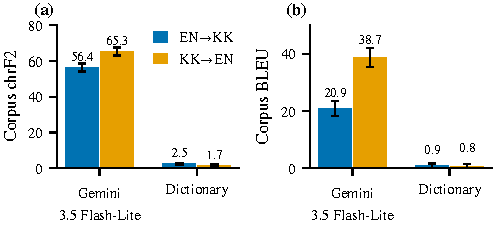
\includegraphics[width=\columnwidth]{figures/fig_direction.pdf}
\caption{Corpus (a) chrF2 and (b) BLEU by translation direction on the same \NPairs{} FLORES-200 items. Error bars are 95\% paired bootstrap intervals (\NBoot{} resamples, seed 42).}
\label{fig:direction}
\end{figure}

\subsection{Item-Level Evidence}
The corpus gap is not driven by a few items. Translation into Kazakh scored lower on \ItemsBelow{} of \NPairs{} items (\ItemsBelowPct\%; Fig.~\ref{fig:paired}a), and the median per-item difference was $\WilMed$ chrF2 points (Fig.~\ref{fig:paired}b). The Wilcoxon signed-rank test rejected equality of the paired sentence scores ($W=\WilW$, $p_{\mathrm{Holm}}=\WilP$) with a medium-to-large effect ($r_{\mathrm{rb}}=\WilR$; Table~\ref{tab:tests}). The two comparisons against the dictionary baseline were also significant in both directions. Item-level variation is nevertheless large: some items scored higher into Kazakh, and the three outputs written mainly in Latin script appear as clear outliers near zero.

\begin{figure}[!t]
\centering
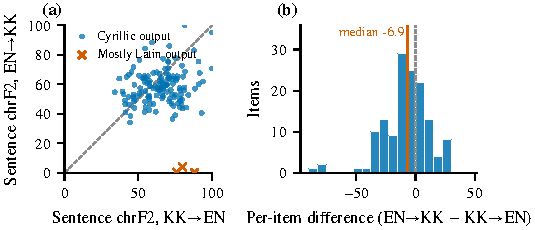
\includegraphics[width=\columnwidth]{figures/fig_paired.pdf}
\caption{(a) Sentence-level chrF2 of each item in both directions; points below the diagonal scored lower into Kazakh, and crosses mark outputs written mainly in Latin script. (b) Distribution of per-item differences; the orange line marks the median.}
\label{fig:paired}
\end{figure}

\begin{table}[!t]
\centering
\caption{Wilcoxon Signed-Rank Tests on Paired Sentence chrF2 ($n=\NPairs$). $\Delta$ Follows the Order Shown; $r_{\mathrm{rb}}$ Is the Matched-Pairs Rank-Biserial Correlation.}
\label{tab:tests}
\footnotesize
\resizebox{\columnwidth}{!}{\begin{tabular}{@{}lrrrr@{}}
\toprule
Comparison & Median $\Delta$ & $W$ & $p_{\mathrm{Holm}}$ & $r_{\mathrm{rb}}$ \\
\midrule
Gemini: EN$\rightarrow$KK vs.\ KK$\rightarrow$EN & -6.90 & 2564 & $2.1\times10^{-6}$ & -0.47 \\
Gemini vs.\ dictionary, EN$\rightarrow$KK & +54.62 & 3 & $6.5\times10^{-24}$ & +1.00 \\
Gemini vs.\ dictionary, KK$\rightarrow$EN & +64.38 & 0 & $6.5\times10^{-24}$ & +1.00 \\
\bottomrule
\end{tabular}
}
\end{table}

\subsection{Robustness and Sensitivity}
Table~\ref{tab:robust} and Fig.~\ref{fig:forest} show that the direction of the gap does not depend on the metric or on the analysed subset. chrF++ ($\GemChrfPPGap$), BLEU ($\GemBleuGap$) and TER ($+\GemTerGap$, where higher is worse) all indicate lower quality into Kazakh, and all four intervals exclude zero. Removing the \NPilotOverlap{} items that overlap the pilot set changed the chrF2 gap by less than 0.03 points ($\GapNoPilot$, $[\GapNoPilotLo, \GapNoPilotHi]$). Removing the \NMostlyLatin{} mostly Latin-script outputs reduced the gap to $\GapNoLatin$ ($[\GapNoLatinLo, \GapNoLatinHi]$), so script errors explain part, but clearly not most, of the difference. The gap was negative in all three FLORES domains and in all three source-length groups; the interval for short sources (up to \LenCutLo{} words) included zero. These subgroup estimates are exploratory and their intervals overlap. Source length was only weakly associated with sentence chrF2 (Spearman $\rho=\RhoLenKK$ into Kazakh, $\RhoLenEN$ into English).

\begin{table}[!t]
\centering
\caption{Robustness of the Directional Gap. Gaps With 95\% Paired Bootstrap Intervals. $^{\dagger}$For TER, Lower Is Better, so a Positive Gap Indicates Lower Quality Into Kazakh.}
\label{tab:robust}
\footnotesize
\begin{tabular}{@{}lrcc@{}}
\toprule
Analysis & $n$ & Gap & 95\% CI \\
\midrule
\multicolumn{4}{@{}l}{\textit{Metric (all pairs)}} \\
chrF2 (primary) & 138 & $-$8.93 & [$-$12.19, $-$5.64] \\
chrF++ & 138 & $-$11.28 & [$-$14.50, $-$7.92] \\
BLEU & 138 & $-$17.84 & [$-$21.83, $-$13.84] \\
TER$^{\dagger}$ & 138 & +18.55 & [13.93, 23.02] \\
\multicolumn{4}{@{}l}{\textit{Sensitivity (chrF2)}} \\
Pilot items removed & 124 & $-$8.91 & [$-$12.51, $-$5.48] \\
Latin-script outputs removed & 135 & $-$7.28 & [$-$10.00, $-$4.27] \\
\multicolumn{4}{@{}l}{\textit{Subgroup (chrF2, exploratory)}} \\
Domain: wikibooks & 49 & $-$6.50 & [$-$10.19, $-$2.50] \\
Domain: wikinews & 46 & $-$12.39 & [$-$18.39, $-$6.42] \\
Domain: wikivoyage & 43 & $-$7.83 & [$-$14.83, $-$1.69] \\
Length: short & 48 & $-$4.37 & [$-$10.14, 1.14] \\
Length: medium & 46 & $-$13.89 & [$-$19.60, $-$8.19] \\
Length: long & 44 & $-$7.76 & [$-$13.02, $-$3.44] \\
\bottomrule
\end{tabular}

\end{table}

\begin{figure}[!t]
\centering
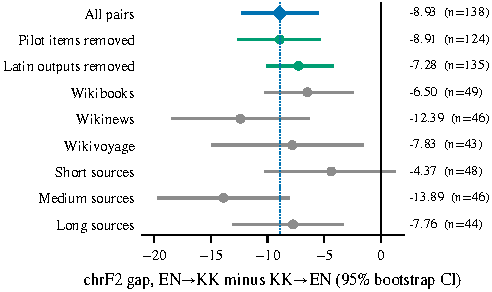
\includegraphics[width=\columnwidth]{figures/fig_forest.pdf}
\caption{chrF2 gap (EN$\rightarrow$KK minus KK$\rightarrow$EN) with 95\% bootstrap intervals for all pairs (blue), the planned sensitivity analyses (green) and exploratory subgroups (grey). The dotted line marks the overall estimate.}
\label{fig:forest}
\end{figure}

\subsection{Diagnostic 1: Script}
Of the \NPairs{} Kazakh outputs, \NMostlyLatin{} were written mainly in Latin-script Kazakh and \NAnyLatin{} contained at least one Latin letter. Latin letters are not errors in themselves: \NRefLatin{} of the professional Kazakh references also contain Latin characters, typically names, units or abbreviations such as ``pH''. The mostly Latin outputs, however, score near zero chrF2 against Cyrillic references even when parts of them are readable, because character n-grams cannot match across scripts.

\subsection{Diagnostic 2: Inflection-Tolerant Matching}
Exact word recall against the reference was much lower for Kazakh outputs (\RecallKK\%) than for English outputs (\RecallEN\%). Fig.~\ref{fig:inflection} shows how many additional reference words are matched when words are compared by their first $k$ letters. At $k=\KPrimary$, \NmKK\% of Kazakh reference words (95\% CI $[\NmKKLo, \NmKKHi]$) were matched only at the prefix level, compared with \NmEN\% ($[\NmENLo, \NmENHi]$) of English ones, a difference of \NmDiff{} percentage points ($[\NmDiffLo, \NmDiffHi]$). The mismatched-reference control produced only \NmCtrlKK\% and \NmCtrlEN\%, so chance prefix collisions do not explain the pattern. Put differently, about \NmShareOfMissKK\% of the Kazakh reference words that the model did not reproduce exactly appeared in the output with the same five-letter beginning but a different ending, against \NmShareOfMissEN\% in English. The Kazakh excess was present at every prefix length from 3 to 8.

\begin{figure}[!t]
\centering
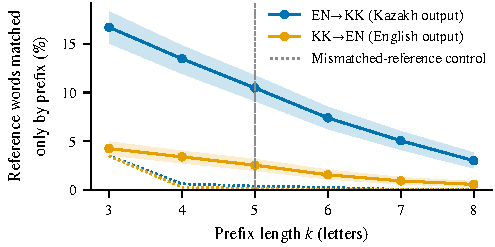
\includegraphics[width=\columnwidth]{figures/fig_inflection.pdf}
\caption{Share of reference words matched only after both texts are cut to $k$-letter prefixes (same beginning, different ending), with 95\% bootstrap bands. Dotted lines show the mismatched-reference control. The dashed vertical line marks the main setting $k=\KPrimary$.}
\label{fig:inflection}
\end{figure}

Table~\ref{tab:ablation} reports the corresponding ablation. Cutting all words to five letters shrank the BLEU gap from $\AblBleuGapFull$ to $\AblBleuGapK$ (\AblBleuRedPct\% smaller) and the word-F1 gap from $\AblFoneGapFull$ to $\AblFoneGapK$ (\AblFoneRedPct\% smaller), whereas the chrF2 gap was essentially unchanged ($\AblChrfGapK$). Word-level metrics thus overstate the Kazakh deficit partly because they treat every suffix difference as a complete miss, while chrF2 already gives partial credit for shared stems. The substantial gap that remains after truncation indicates that differences beyond word endings---lexical choices, omissions, additions and reordering---also contribute.

\begin{table}[!t]
\centering
\caption{Ablation: Directional Gaps After Cutting Every Word in Outputs and References to Its First $k$ Letters ($n=\NPairs$).}
\label{tab:ablation}
\footnotesize
\begin{tabular}{@{}lccc@{}}
\toprule
Word form & chrF2 gap & BLEU gap & Word-F1 gap \\
\midrule
Full forms & -8.93 & -17.84 & -22.01 \\
6-letter prefix & -9.10 & -14.19 & -16.31 \\
5-letter prefix & -9.00 & -13.24 & -14.28 \\
4-letter prefix & -8.82 & -12.38 & -12.19 \\
\bottomrule
\end{tabular}

\end{table}

\subsection{Diagnostic 3: Token Usage}
For translations of the same \NPairs{} source sentences, Kazakh outputs consumed \TokRatio{} times as many output tokens as English outputs (95\% CI $[\TokRatioLo, \TokRatioHi]$), although they were only \CharRatio{} times as long in characters. Per character, Kazakh required \TokPerCharKK{} tokens per 100 characters against \TokPerCharEN{} for English, a premium of \TokCharPrem$\times$ ($[\TokCharPremLo, \TokCharPremHi]$; Fig.~\ref{fig:tokens}a). The input side gave a consistent estimate: regressing prompt tokens on source length in both directions yielded \TokSrcRatio{} times as many tokens per character for Kazakh sources. At the level of individual items, the token ratio was not associated with the chrF2 gap (Spearman $\rho=\RhoTok$, $p=\RhoTokP$; Fig.~\ref{fig:tokens}b). Tokenization therefore represents a consistent cost burden for Kazakh, but within this sample it does not predict which sentences are translated worse. Median request latency was \LatKK{}~s into Kazakh and \LatEN{}~s into English; because latency includes the public network path, we do not interpret it further.

\begin{figure}[!t]
\centering
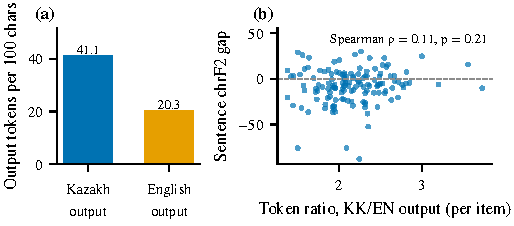
\includegraphics[width=\columnwidth]{figures/fig_tokens.pdf}
\caption{(a) Visible output tokens per 100 characters reported by the Gemini API for the same \NPairs{} items. (b) Per-item ratio of Kazakh to English output tokens against the per-item chrF2 gap.}
\label{fig:tokens}
\end{figure}

\subsection{Question Answering Calibration}
No model QA responses have been saved yet, so H1 for QA cannot be tested. Table~\ref{tab:qa} reports the two language-blind rules on all \NQa{} paired Belebele questions. Always answering~A scored \QaAKK\% in both languages. A single seeded random guesser scored \QaRndKK\% in Kazakh and \QaRndEN\% in English, with \QaRndKKonly{} items correct only in Kazakh and \QaRndENonly{} only in English (exact McNemar $p=\QaRndP$). An 8.5-point difference can therefore arise from a rule that uses no language information at all, which shows why paired tests on discordant items, rather than raw accuracy differences, are required for the model comparison.

\begin{table}[!t]
\centering
\caption{QA Accuracy on \NQa{} Paired Belebele Questions With Exact 95\% Intervals, Discordant Pairs and Exact McNemar $p$-Values}
\label{tab:qa}
\footnotesize
\resizebox{\columnwidth}{!}{\begin{tabular}{@{}lccrr@{}}
\toprule
Condition & Kazakh (\%) & English (\%) & KK/EN only & $p$ \\
\midrule
Always A & 19.5 {\scriptsize[14.2, 25.7]} & 19.5 {\scriptsize[14.2, 25.7]} & 0/0 & 1.000 \\
Seeded random & 18.5 {\scriptsize[13.4, 24.6]} & 27.0 {\scriptsize[21.0, 33.7]} & 29/46 & 0.064 \\
Gemini 3.5 Flash-Lite & \multicolumn{4}{c}{\textit{pending: no QA responses saved}} \\
Qwen 2.5 1.5B & \multicolumn{4}{c}{\textit{pending: no QA responses saved}} \\
Gemma 3 & \multicolumn{4}{c}{\textit{pending: no QA responses saved}} \\
\bottomrule
\end{tabular}
}
\end{table}

\subsection{Qualitative Review of Low-Scoring Outputs}
To illustrate what the scores penalise, the \NReviewed{} Kazakh outputs with the lowest sentence chrF2 received provisional labels in an AI-assisted first pass that the authors reviewed against the source and the output (Table~\ref{tab:labels}). This is a single, unblinded pass on a sample selected for low scores, so its proportions describe the tail and not Kazakh output in general, and it does not substitute for the planned blind annotation. The most frequent outcome (\LabReferenceMismatch{} of \NReviewed) was a plausible translation phrased differently from the single reference, which confirms that low chrF2 does not always mean a wrong translation. Lexical problems (\LabLexical) included non-words such as \kk{беінші}{beinshi} for \kk{бесінші}{besinshi} (``fifteenth'') and Russian spellings such as \kk{Цыган}{Tsygan} for Kazakh \kk{Сыған}{Syghan}. Semantic problems (\LabSemantic) included rendering ``worked to death'' as ``tortured to death''. The \LabScript{} script cases were whole sentences in Latin-script Kazakh. Only \LabMorphological{} case was labelled primarily morphological (\kk{әрпи}{ärpiy} instead of the possessive form \kk{әрпі}{ärpi}); because each case received a single primary label, suffix errors that co-occur with lexical problems are not counted separately.

\begin{table}[!t]
\centering
\caption{First-Pass Labels of the \NReviewed{} Lowest-chrF2 EN$\rightarrow$KK Outputs (Provisional AI-Assisted Pass Reviewed by the Authors; Blind Double Annotation Pending)}
\label{tab:labels}
\footnotesize
\begin{tabular}{@{}lrr@{}}
\toprule
First-pass label & Count & Share (\%) \\
\midrule
Reference mismatch & 13 & 43.3 \\
Lexical & 9 & 30.0 \\
Semantic & 4 & 13.3 \\
Script & 3 & 10.0 \\
Morphological & 1 & 3.3 \\
\midrule
Total & 30 & 100.0 \\
\bottomrule
\end{tabular}

\end{table}

\section{Discussion}
\label{sec:discussion}

\subsection{Answer to the Research Question}
For the evaluated model and data, translation quality is clearly lower when the model writes Kazakh than when it writes English. The gap of $\GemChrfGapAbs$ chrF2 points is large relative to its uncertainty, appears in about two thirds of individual items, and keeps its direction under four metrics and three sensitivity analyses. Table~\ref{tab:hyp} summarises the status of each hypothesis against the criteria fixed in the protocol. H1 is supported for the translation contrast of one model, but the protocol also requires the gap to exceed that of a dedicated translation system, and this NLLB comparison is pending. H1 for QA and H2, which is defined on blind human annotations, cannot yet be evaluated.

\begin{table}[!t]
\centering
\caption{Status of the Hypotheses Against the Protocol Criteria}
\label{tab:hyp}
\footnotesize
\begin{tabular}{@{}p{2.0cm}p{3.4cm}p{2.3cm}@{}}
\toprule
Claim & Evidence & Status \\
\midrule
H1, translation & $\gap_{\mathrm{chrF2}}=\GemChrfGap$, CI below zero; robust to metric and subset & Supported for Gemini; NLLB-relative test pending \\
H1, QA & No saved model QA responses & Pending \\
H2, morphology largest & Automatic near-miss excess of \NmDiff{} pp; human labels provisional & Not testable yet; automatic evidence consistent \\
\bottomrule
\end{tabular}
\end{table}

\subsection{What the Diagnostics Show}
The diagnostics decompose the gap into parts that can be measured without human labels. Script errors are real but rare: excluding three Latin-script outputs moves the gap by about 1.6 points. Suffix-level mismatch is common: one in ten Kazakh reference words is reproduced with the right beginning but a different ending, four times the English rate, and the mismatched-reference control rules out chance. This pattern is what agglutinative morphology predicts, because a Kazakh word form bundles case, possession and number into suffixes that the model can choose differently from the reference translator, sometimes correctly and sometimes not. The ablation adds a methodological point: BLEU and word-level F1 shrink substantially when suffixes are ignored, whereas chrF2 does not, which supports the protocol's choice of chrF2 as the primary metric for Kazakh and cautions against comparing word-level scores across languages with different morphology~\cite{kocmi2021ship,popovic2015chrf}. Finally, the remaining gap after truncation and the qualitative review both point to lexical and semantic differences as further contributors.

Near-miss matches are not necessarily errors. A different case ending can be an equally valid choice under a different sentence structure, and the review found that most low-scoring outputs were acceptable paraphrases. The diagnostic therefore measures where the model's word forms \emph{diverge} from the reference, not how often they are wrong; the blind annotation is needed to estimate the latter.

\subsection{Comparison With Prior Studies}
The direction of our result agrees with large multilingual studies that find general LLMs weaker for lower-resource languages~\cite{robinson2023chatgpt,zhu2024multilingual,ahuja2023mega}, and with Kazakh-specific evaluations reporting Kazakh deficits for LLMs~\cite{togmanov2025kazmmlu,maxutov2024kazakh}. Our study differs from these in holding content constant and in testing explanations. Yeshpanov et al.\ attributed weaker scores into Kazakh to agglutinative morphology without a direct test~\cite{yeshpanov2024kazparc}; the prefix analysis provides automatic evidence consistent with that explanation and shows that it is incomplete. Petrov et al.\ reported that the GPT-4 tokenizer needs several times more tokens for Kazakh than for English~\cite{petrov2023tokenizer}; we measured a premium of about two for the Gemini API on output and input text. The measurements are not directly comparable because they use different tokenizers and normalisations, but both indicate that Kazakh users pay more per unit of content, in line with Ahia et al.~\cite{ahia2023cost}. Unlike Rust et al.'s observation that tokenizer quality relates to downstream performance across languages~\cite{rust2021tokenizer}, we found no item-level association between token ratio and score within one language pair, which suggests that tokenization cost and translation quality should be treated as separate problems. The prominence of reference variation in the low-scoring tail echoes the finding of Freitag et al.\ that expert error analysis can change conclusions drawn from automatic metrics~\cite{freitag2021experts}.

\subsection{Practical Implications}
For users, the results suggest checking three things in LLM output into Kazakh: the script, the endings of inflected words, and names and numerals, where several lexical errors occurred. For developers, the near-miss rate is a cheap, reference-based signal that can be tracked across model versions together with token cost. For evaluators of Kazakh systems, character-level metrics, paired designs and significance tests on discordant items are preferable to raw word-level scores or unpaired accuracy differences, as the random-guessing calibration in Table~\ref{tab:qa} illustrates.

\subsection{Threats to Validity}
\paragraph*{Internal validity} Pairing holds content constant, but direction also changes the source language and the nature of the reference. FLORES-200 sentences were written in English and translated into Kazakh, so in the \KKEN{} direction the model translates translated Kazakh back towards an original English sentence, while in the \ENKK{} direction it is compared with one translator's Kazakh rendering. Both effects could favour the English direction independently of model ability. The KazParC items, which come from Kazakh-centred sources, and the NLLB baseline are the planned controls for this threat; both are pending. Provider-side model updates between requests cannot be excluded, although all responses were collected on one day and report the same model version.

\paragraph*{Construct validity} chrF2 measures surface overlap with a single reference, not adequacy. Character n-grams in an agglutinative language and in English are not strictly commensurate, which is why the protocol interprets the LLM gap relative to a dedicated system's gap. Script mismatches can drive scores to near zero for readable output. The near-miss diagnostic uses fixed-length prefixes as a proxy for stems; it cannot distinguish valid from invalid inflection and may count unrelated words that share a beginning, although the control shows that such collisions are rare at $k=5$.

\paragraph*{External validity} The evidence concerns one model and version, one provider, zero-shot prompts and three FLORES-200 domains. It does not establish how other models, Kazakh-original text, longer documents or QA behave. FLORES-200 is public, so prior exposure during pretraining is possible~\cite{sainz2023contamination}; the team-written probes, intended as a clean check, have no outputs yet.

\paragraph*{Statistical conclusion validity} The bootstrap treats items as independent, although some FLORES sentences come from the same article. Intervals are conditional on one saved generation per prompt and do not capture variation between runs. Subgroup analyses are exploratory and uncorrected. The saved items are the first \NPairs{} FLORES pairs in collection order rather than a random subset of the benchmark, so coverage was determined by when collection stopped.

\subsection{Limitations}
The main limitation is incomplete coverage: one third of one model's planned responses, no QA or probe responses, no second or third model, no NLLB baseline and no blind annotation with inter-annotator agreement~\cite{cohen1960}. The test set also contains all pilot items, so a fully independent evaluation set is not available; the pilot-exclusion analysis shows that removing the overlapping translation items barely changes the estimate, but it cannot undo earlier exposure. These limitations restrict the scope of the conclusions, not their validity within that scope, and each can be removed by running the released pipeline without protocol changes.

\section{Conclusion}
\label{sec:conclusion}

This article asked how LLM performance on Kazakh compares with performance on equivalent English tasks and which linguistic properties accompany any difference. Using a paired, hash-frozen benchmark and an auditable pipeline, we found that Gemini 3.5 Flash-Lite translates into Kazakh markedly worse than into English on the same \NPairs{} FLORES-200 sentences: the chrF2 gap of $\GemChrfGap$ points has a paired 95\% interval of $[\GemChrfGapLo, \GemChrfGapHi]$ and is robust across metrics, pilot exclusion and script exclusion. Three diagnostics explain part of the difference. Script errors are rare and account for a small share of the gap; suffix-level divergence from the reference is four times as frequent in Kazakh as in English and is not explained by chance prefix matches; and Kazakh text costs about twice as many tokens per character, a burden that does not, however, predict item-level quality.

The contributions are the released benchmark and pipeline, a statistically rigorous directional comparison, and controlled automatic diagnostics that turn the morphology hypothesis into a measurable quantity. Future work will complete the protocol: the remaining Gemini prompts, Qwen~2.5 and Gemma~3, the NLLB-200 reference gap, question answering with exact McNemar tests, the 30 probes, and blind double annotation with agreement statistics to test H2 directly. Adding Kazakh-original evaluation text and a genuinely separate test set will address the main threats to validity identified here.

\section*{Data and Code Availability}
The benchmark, saved model responses, analysis code, generated results and the source of this article are available at \url{https://github.com/tw3tyy/kazllm} under the MIT licence (code) and the original CC BY-SA 4.0 and CC BY 4.0 licences (benchmark sources). The release tagged \texttt{final} corresponds to this version; [Zenodo DOI to be added after archiving the release]. Running \texttt{python3 -m paper.analysis.run} regenerates every table, figure and number reported here. API keys are not stored, and the saved responses contain no personal data.

\section*{Author Contributions (CRediT)}
[To be confirmed by all authors before submission.] \textbf{B.~Kazhymukhamet:} Conceptualization, Methodology, Software, Formal analysis, Visualization, Writing -- original draft. \textbf{M.~Khaigeldinova:} Data curation, Investigation, Validation, Writing -- review \& editing. \textbf{D.~Bekbosyn:} Data curation, Investigation, Resources, Writing -- review \& editing. All authors read and approved the final manuscript.

\section*{Use of Generative AI}
In line with IEEE policy and the course rules, the authors disclose that a generative AI assistant ([name and version of the tool]) was used to review and extend the analysis code, to draft provisional first-pass labels for the qualitative review in Section~\ref{sec:results}, and to edit the language of the manuscript. The authors checked all code, outputs, labels, references and text, and take full responsibility for the content. The AI tool is not an author. Gemini 3.5 Flash-Lite appears in this article only as the system under evaluation.

\section*{Conflict of Interest}
The authors declare no conflict of interest.

\section*{Funding}
This research received no external funding. Model access used free API tiers and local hardware.

\section*{Ethics Statement}
The study did not involve human participants, personal data or animal subjects, and therefore did not require ethical approval. Error annotation is performed by the authors themselves.

\section*{Acknowledgment}
The authors thank the School of Software Engineering at Astana IT University and the instructors of the Research Methods and Tools course for feedback on the study protocol.


\bibliographystyle{IEEEtran-doi}
\bibliography{references}

\end{document}
